\newpage
\section{Display}
	The display is one of the main parts of the ArticlePlaceholder, as it is user-facing and therefore needs an initial default design. \\
	\begin{figure}[H]
		\centering
		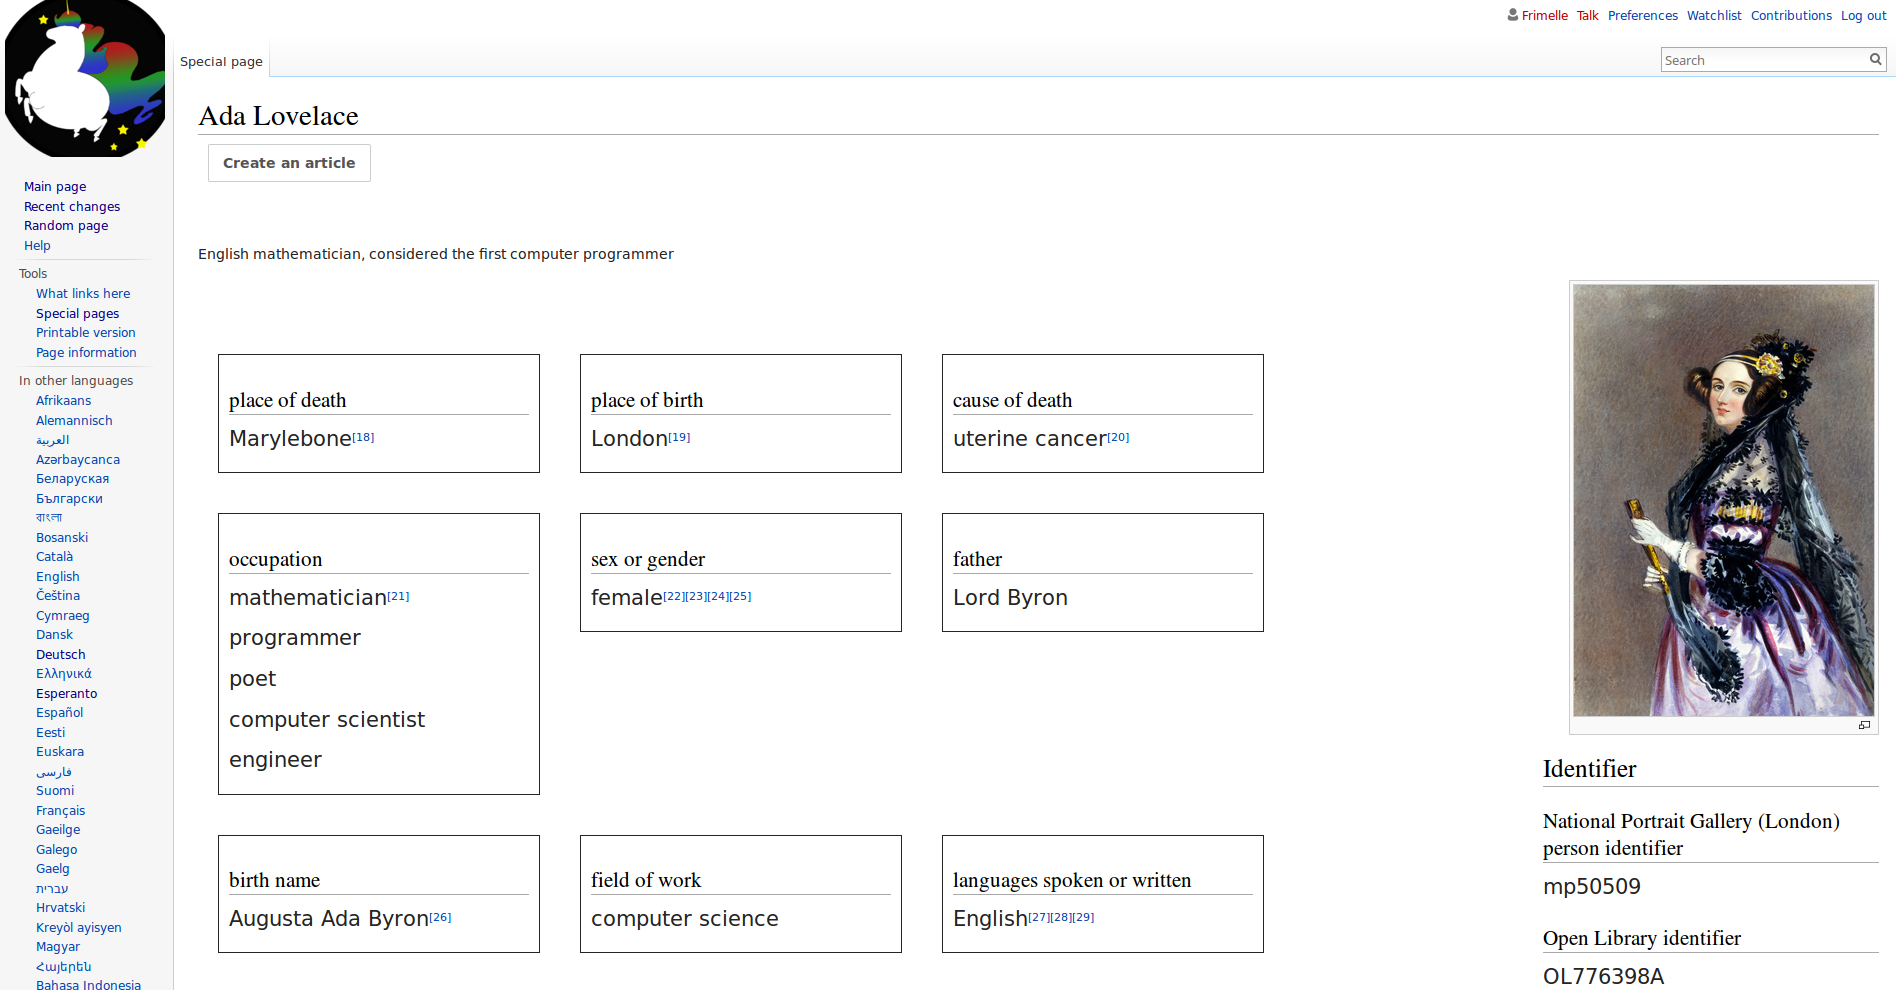
\includegraphics[width=\textwidth]{diagrams/Screenshot-ArticlePlaceholder.png}
		\caption{Screenshot of the ArticlePlaceholder layout as of January 2016}
		\label{screenshot}
	\end{figure}
	The core part of the page is formed by the statement groups. These consist of a property, one or multiple values, and their qualifiers. \\
	Each statement group is in a box with a black border and arranged in a tile layout. The number of statement boxes per row differs depending on the width of the screen. \\
	\begin{figure}[H]
		\centering
		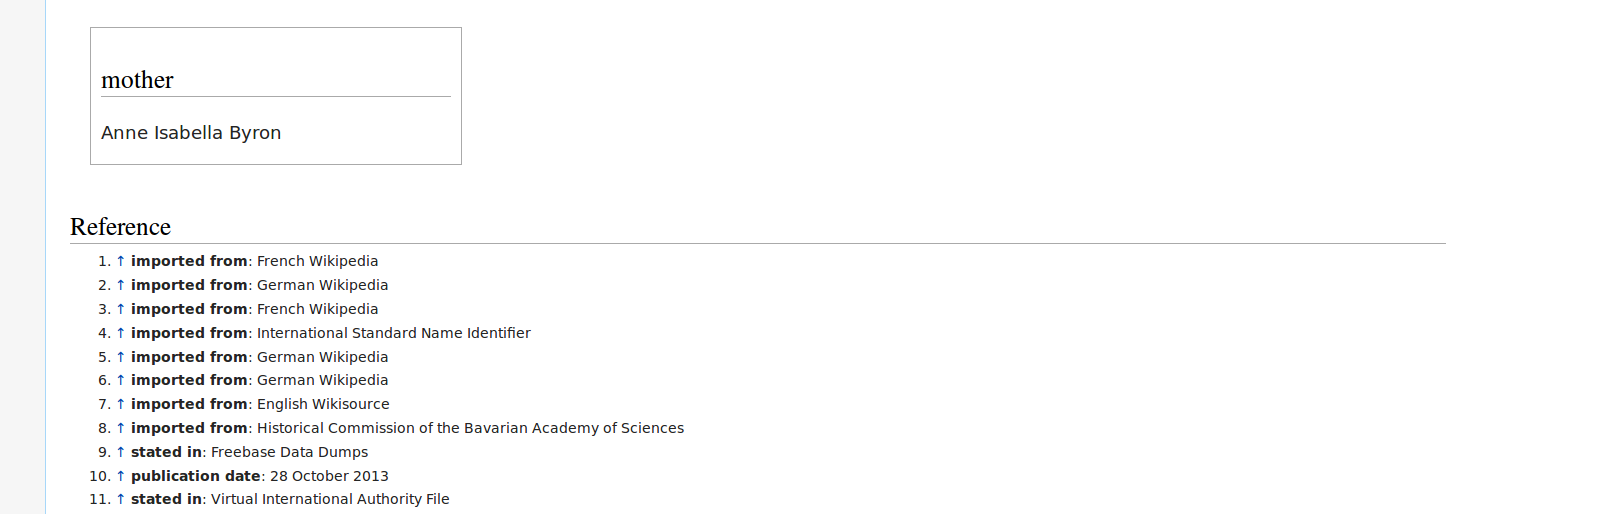
\includegraphics[width=\textwidth]{diagrams/references.png}
		\caption{Screenshot of the ArticlePlaceholder layout, Reference section as of January 2016}
		\label{fig:references}
	\end{figure}
	The main image of the item is on the right side (for left to right languages) of the page, where it would also be in articles.\\
	The label of the property is the header for each group, which is separated from the body by a horizontal line. Multiple values for the same statement are also separated by a line. Their qualifiers are directly under the corresponding value. \\
	References can be found in their own section at the bottom of the page, conforming to the existing layout of Wikipedia, see Figure~\ref{fig:references}. \\
	The identifier of an item should be in a distinct position so as to be both emphasized and distinguishable from the other statements. They are listed below the main image of the article to the right of the statement groups.
	
	\subsection{Renderer}

Every part of an entity, or item in the case of the ArticlePlaceholder, needs a \textit{renderer} to be displayed. The renderer are written in Lua. They pull data from Wikidata and render it to HTML. They set CSS classes for the HTML elements in order to style them with the CSS module \texttt{\justify ext.articleplaceholder.defaultDisplay.css}. The HTML output of the module is displayed on the \texttt{\justify Special:AboutTopic} ArticlePlaceholder. \\
The MediaWiki conventions for naming Lua modules is 
\begin{center}
\texttt{\justify mw.ext.extensionName.moduleName} 
\end{center}
In order to match them, the default renderer for ArticlePlaceholders is called 
\begin{center}
\texttt{\justify mw.ext.articlePlacholder.entityRenderer}
\end{center}
The entity renderer has getter and setter functions for individual renderers. Therefore every part of the display logic can be overwritten locally on Wikipedia. \\
The Lua module on the Wikipedia is at \texttt{\justify Module:AboutTopic}, which is invoked by \texttt{\justify Template:AboutTopic}. On the entity renderer instance obtained a user with the appropriate rights can call the getter and setter functions. \\
The renderer are as interchangeable as possible so that for example the \texttt{\justify snaksRenderer} can be used by the \texttt{\justify refererenceRenderer} as well as the \texttt{\justify qualifierRenderer}. The scopes of the renderer are therefore limited to their functionality. \\
Wikibase provides a Scribunto interface with functions to access the repository. Wherever possible, the functions provided by this interface were used. This way, the description renderer for example simply wraps \texttt{\justify mw.wikibase.description}. The \texttt{\justify descriptionRenderer} of the ArticlePlacheolder's EntityRenderer is still needed as a seperate service since there must be a possibility for the user to overwrite the renderer. Additionally a CSS class is wrapped around the result of Wikibase's description renderer in order to style it properly. \\
The EntityRenderer module itself takes the entity Id of an item an ArticlePlaceholder is created for. The Lua table for an entity is loaded in the \texttt{\justify renderEntity} function. This table represents the whole entity with all its respective data. Therefore it is performance-wise a very expensive operation. \\

\begin{figure}[H]
	\centering
	\includegraphics[width=\textwidth]{diagrams/EntityRendererMethods.png}
	\caption{Diagram of all renderer functions}
	\label{fig:renderer}
\end{figure}
	\documentclass[11pt]{article}

\usepackage[dvipsnames]{xcolor}
\usepackage{hyperref}
\usepackage{todonotes}
\usepackage{listings}

\title {{Functional requirements}}
\author {Lucie-Aim\'{e}e Kaffee}
\date{}

\begin{document}

\section{Identifier}

To get a list of all external identifier in Wikidata, the item Q19847637, "Wikidata property representing a unique identifier", was used. To get all the Items, that were an instance of (property P31) this item, I used  \href{https://query.wikidata.org}{Wikidata's SPARQL endpoint}. A file with the property Ids is returned. The JSON format was the most useful in this case to be converted to a Lua table. \\

\begin{lstlisting}[frame=single] 
PREFIX wd: <http://www.wikidata.org/entity/>
PREFIX wdt: <http://www.wikidata.org/prop/direct/>

SELECT ?identifier WHERE {
   ?identifier  wdt:P31 wd:Q19847637 . 
}
\end{lstlisting}

\end{document}
	\documentclass[11pt]{article}

\usepackage[dvipsnames]{xcolor}
\usepackage{hyperref}
\usepackage{todonotes}
\usepackage{listings}
\usepackage{soul}
\usepackage[latin1]{inputenc}
\usepackage{tikz}
\usetikzlibrary{shapes,arrows}

\title {{Implementation}}
\author {Lucie-Aim\'{e}e Kaffee}
\date{}

\begin{document}
Test
\end{document}
	\subsection{Style elemts (CSS)}

In order to style the layout elements, CSS classes were assigned in the Lua module. Their looks as well as the create article button's look are adjusted in \texttt{ext.articleplaceholder.defaultDisplay.css}. The main elements belonging in one part in the layout such as the main image and the identifier, that are in one sidebar, are in one common \texttt{div}. Additionally the identifier are all in one \texttt{div}, the \texttt{sidebar}. \\
To not conflict with other MediaWiki style elements, the CSS classes are prefixed with \texttt{\justify articleplaceholder-}. \\
The \texttt{divs} containing the statement groups have a maximum width, so a maximum of three boxes are in one row. The number of columns differs depend on the amount of statements. When the browser window is smaller, the amount of boxes per row adjusts accordingly. Initially it was planned to adjust them to a tiling layout, but since tiling layout in pure CSS would expect the boxes to be ordered vertically in columns this was not possible. It is important to show the most important information in the first row, otherwise the ordering of statement groups would be pointless. \\
In order to be responsive, the extension makes use of \textit{media queries}. Media queries are a convenient way to add new CSS styles for elements that need to be adjusted for different devices. \citep[43]{mediaquery}\\
In MediaWiki with the \textit{resource loader} \texttt{\justify \$wgResourceModules} media queries can be assigned to CSS modules. This way it is possible to load another CSS module (\texttt{\justify ext.articleplaceholder.defaultDisplaySmall.css}), when the screen size is smaller then 930 pixel. This was mainly added in order to avoid the overlapping of the sidebar with image and identifier, and the statement groups.